% ==================================================
% Appendix: Analysis Systematics %
% ==================================================

%TODO : Organize figure positioning once you're done writing. 

\chapter[Analysis systematics]{Study of systematic uncertainties when using cosmics data for alignment studies}
\label{appendix:systematics}

% Sections:
% 2900 V vs 3100 V 
% Doub gaus vs gaus
% Area bin size
% Residual distribution bin size?

% --------------------------------------------------
\section{Residual distribution fit function}
% --------------------------------------------------
\label{appendix:systematics_res_fit_fcn}

% Edit count: 1

The distribution of residuals should be modeled by a double Gaussian fit\cite{lefebvre_thesis}:

\begin{equation}
\label{eqn:doub_gaus}
G(r) = A_{s}exp\left[ \frac{-(r-\mu)^{2}}{2\sigma_s^{2}} \right] + A_{b}exp\left[ \frac{-(r-\mu)^{2}}{2\sigma_b^{2}} \right]
\end{equation}

where $r$ is the residual, $A$ is the Gaussian amplitude, $\mu$ is the Gaussian mean, $\sigma$ is the Gaussian sigma, and the subscripts $s$ and $b$ stand for signal and background respectively. One Gaussian captures the real (signal) tracks and the other captures the tracks built from noise (background). The Gaussian with the smaller width is identified as the signal. 

A single Gaussian fit failed less often than a double Gaussian fit. The Gaussian fits were performed by initially estimating the amplitude to be 100 tracks, the Gaussian mean to be the histogram mean, and Gaussian $\sigma$ to be the RMS. The fit range was restricted to $\pm$1 root-mean-square (RMS) from the histogram mean. The modification helped the Gaussian fit capture the signal peak. An example residual distribution is shown in Figure~\ref{fig:double_Gaussian_example_fit}. 

\begin{figure}
    \centering
    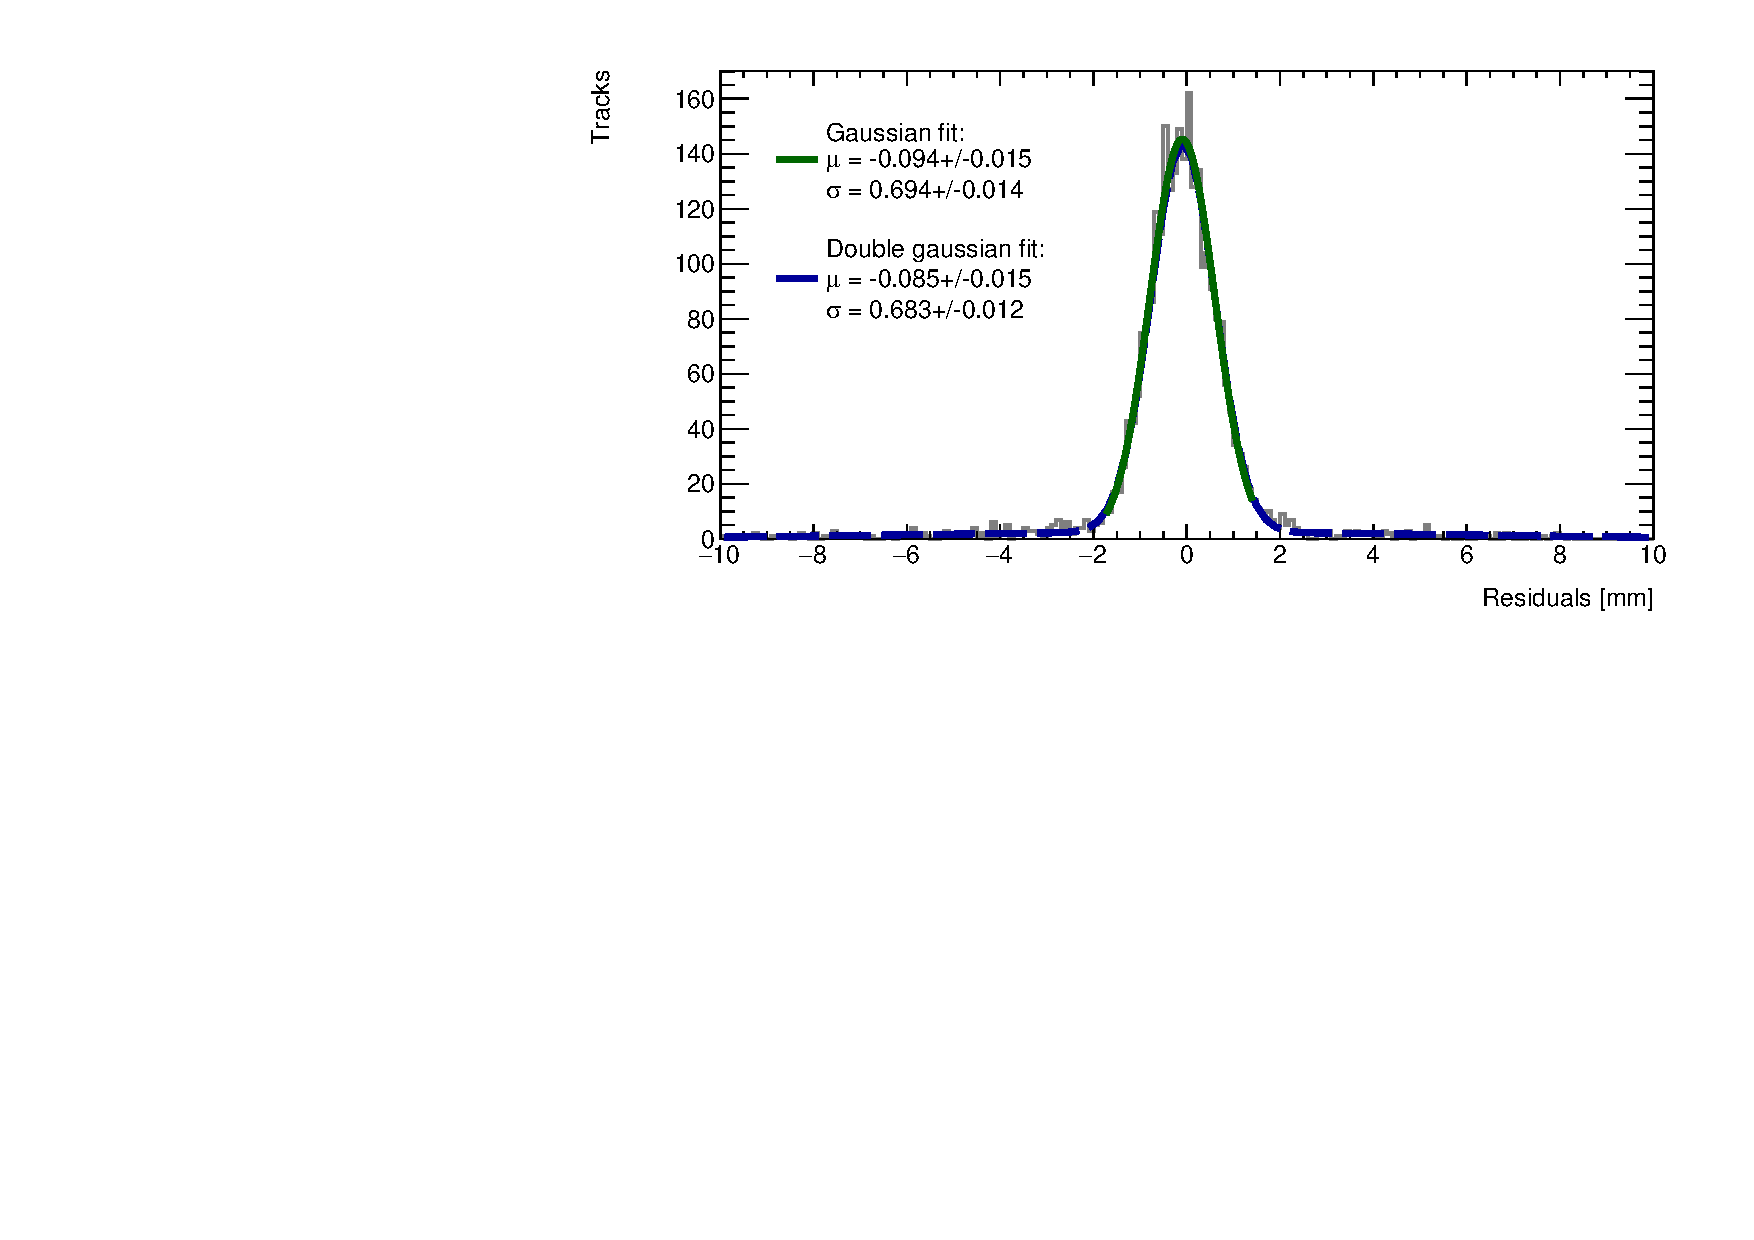
\includegraphics[width = 0.85\textwidth]{figures/figure_double_gaus_vs_gaus_example_fit_QL2P08_3100V_2021-06-18_and_2021-07-19_xbin_10_ybin_5_layer4_fixedlayers12.pdf}
    \caption{Residual distribution for track residuals on layer 4 built from clusters on layers 1 and 2 for $x\in\left[-3.00, 97.00\right]$~mm,  $y\in\left[394.60, 494.60\right]$~mm, fit with a double Gaussian and a single Gaussian in a range of $\pm$1 RMS from the histogram mean.}
    \label{fig:double_Gaussian_example_fit}
\end{figure}

For all residual distributions in \SI{100}{\milli\meter} by \SI{100}{\milli\meter} bins on layer 4 built from clusters on layers 1 and 2, the difference in Gaussian and double Gaussian means and $\sigma$'s is shown in Figure~\ref{fig:double_Gaussian_compare_fits_L4_F12}. The mean of the distribution is centered around zero (within the RMS of the distribution) so the choice of fit algorithm imbues no measurable bias. The order of the RMS is such that the difference in residual means at \SI{40}{\micro\meter} is just significant, so it should be accounted for as a systematic uncertainty on the Gaussian residual means. The \SI{40}{\micro\meter} RMS is for the tracking combination with the worst extrapolation lever arm and the widest distribution of mean differences; the interpolation combinations have narrower distributions, as shown in Figure~\ref{fig:double_Gaussian_compare_fits_L2_F13}. The RMS of the distribution for residual means on layer 2 obtained using reference layers 1 and 3 is only \SI{10}{\micro\meter}, which is almost negligible.

The Gaussian $\sigma$ should be larger than the double Gaussian $\sigma$ because the Gaussian distribution includes the effect of the noise tracks that can yield large residuals, while the double Gaussian models signal and background residuals separately. For this analysis, only the residual mean was important, so the systematic overestimate of the signal $\sigma$ in the Gaussian fit shown in the right-side plots of Figure~\ref{fig:double_Gaussian_compare_fits} was allowed.

\newpage
\thispagestyle{empty}
\newgeometry{top=0.5in,bottom=0.5in}
\begin{figure}
\centering
 \begin{subfigure}{\textwidth}
    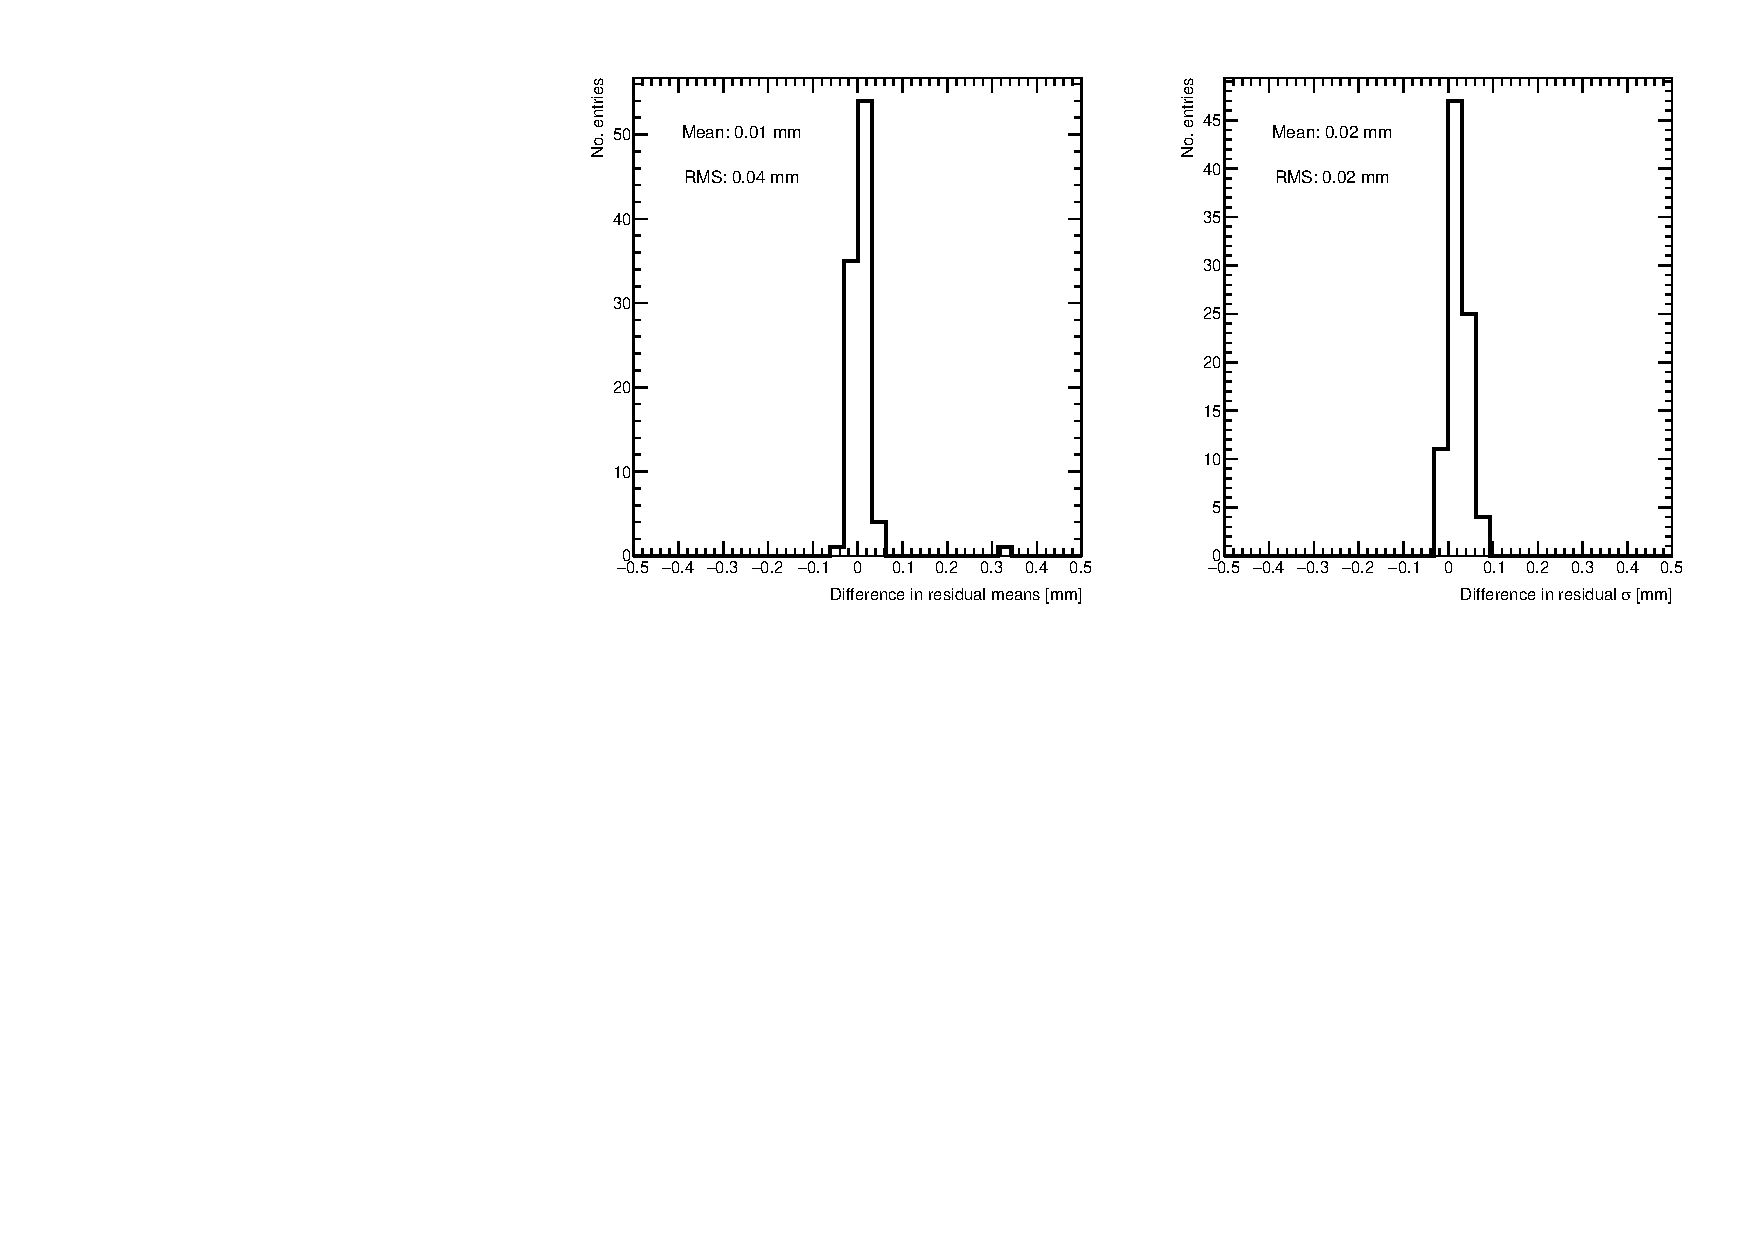
\includegraphics[width = \linewidth]{figures/figure_compare_residual_fits_QL2P08_3100V_2021-06-18_no_dnl_minus_QL2P08_3100V_2021-07-19_doub_gaus_log_scale_layer4_fixedlayers12.pdf} 
    \caption{Difference in residual distribution means (left) and $\sigma$'s (right) extracted with a Gaussian and double Gaussian fit, for all residual distributions in \SI{100}{\milli\meter} by \SI{100}{\milli\meter} bins on layer 4 built from clusters on layers 1 and 2 for sample quadruplet QL2.P.8.}
    \label{fig:double_Gaussian_compare_fits_L4_F12}
  \end{subfigure}
\vspace*{\floatsep}
 
 \begin{subfigure}{\textwidth}
    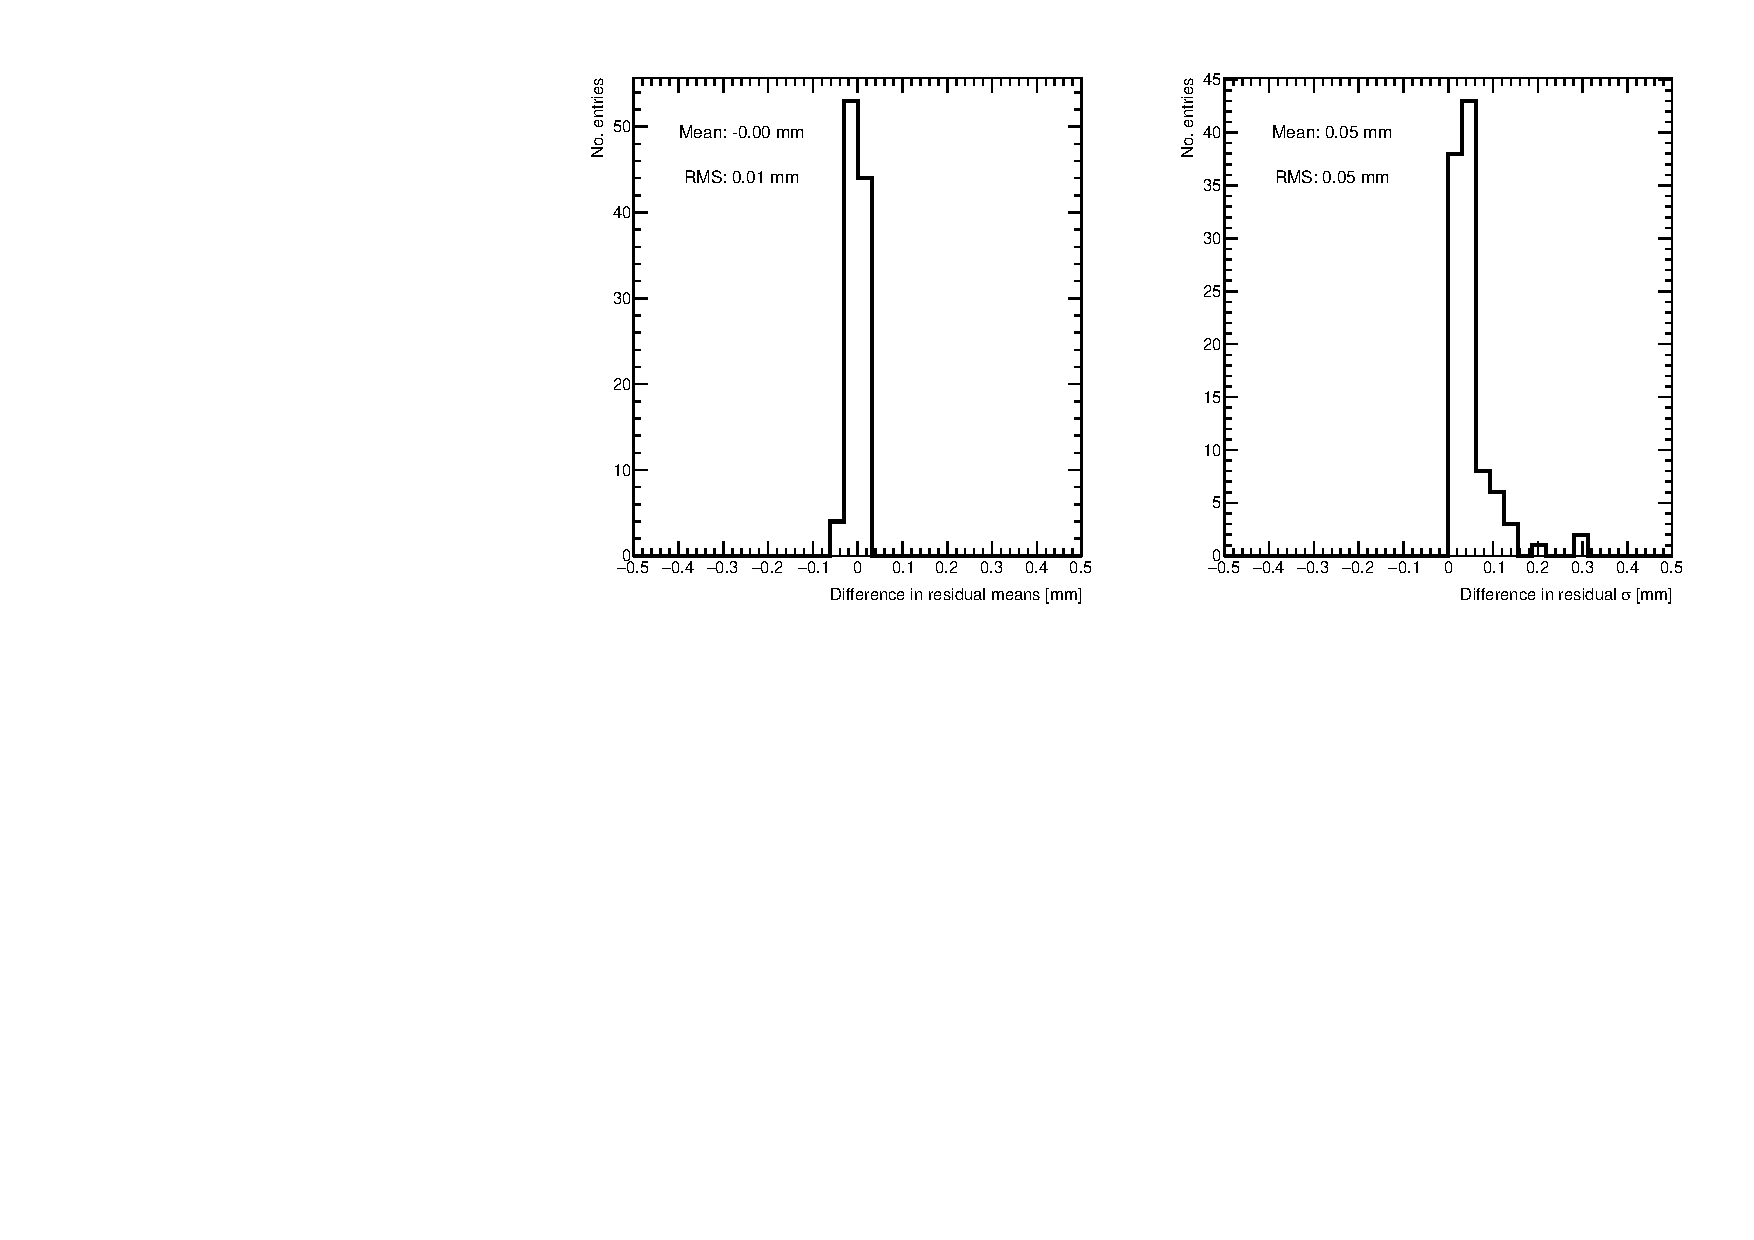
\includegraphics[width = \linewidth]{figures/figure_compare_residual_fits_QL2P08_3100V_2021-06-18_no_dnl_minus_QL2P08_3100V_2021-07-19_doub_gaus_log_scale_layer2_fixedlayers13.pdf} 
    \caption{Difference in residual distribution means (left) and $\sigma$'s (right) for a Gaussian and double Gaussian fit, for all residual distributions in \SI{100}{\milli\meter} by \SI{100}{\milli\meter} bins on layer 2 built from clusters on layers 1 and 3 for sample quadruplet QL2.P.8.}
    \label{fig:double_Gaussian_compare_fits_L2_F13}
  \end{subfigure}
  
  \caption{}
  \label{fig:double_Gaussian_compare_fits}

\end{figure}
\newpage
\restoregeometry

Ultimately, a Gaussian fit was chosen for the track residual distributions because it was more robust and did not affect the fitted mean values too strongly.

% --------------------------------------------------
\section{Cosmic muon data collection voltage}
% --------------------------------------------------
\label{appendix:systematics_2900V_vs_3100V}

% Edit count: 1

Cosmic muon data was collected at 2.9~kV and 3.1~kV because although 2.9~kV is closer to the operating conditions the chambers will be subject to in ATLAS, the extra gain provided by operating at 3.1~kV increased the signal to noise ratio for pad signals. Also, the tracking efficiency was higher with data collected at 3.1~kV. As such, cosmic muon data collected at 3.1~kV was used in the analysis presented in the body of the thesis.

The difference in gain affects the relative population of clusters of different sizes, which in turn affects the uncertainty in the mean cluster positions on each layer, the uncertainty in the track positions and the residual distributions. The residual distributions for 3.1~kV data are narrower, as shown in Figure~\ref{fig:res_dist_2900V_3100V_412}.

\begin{figure}
    \centering
    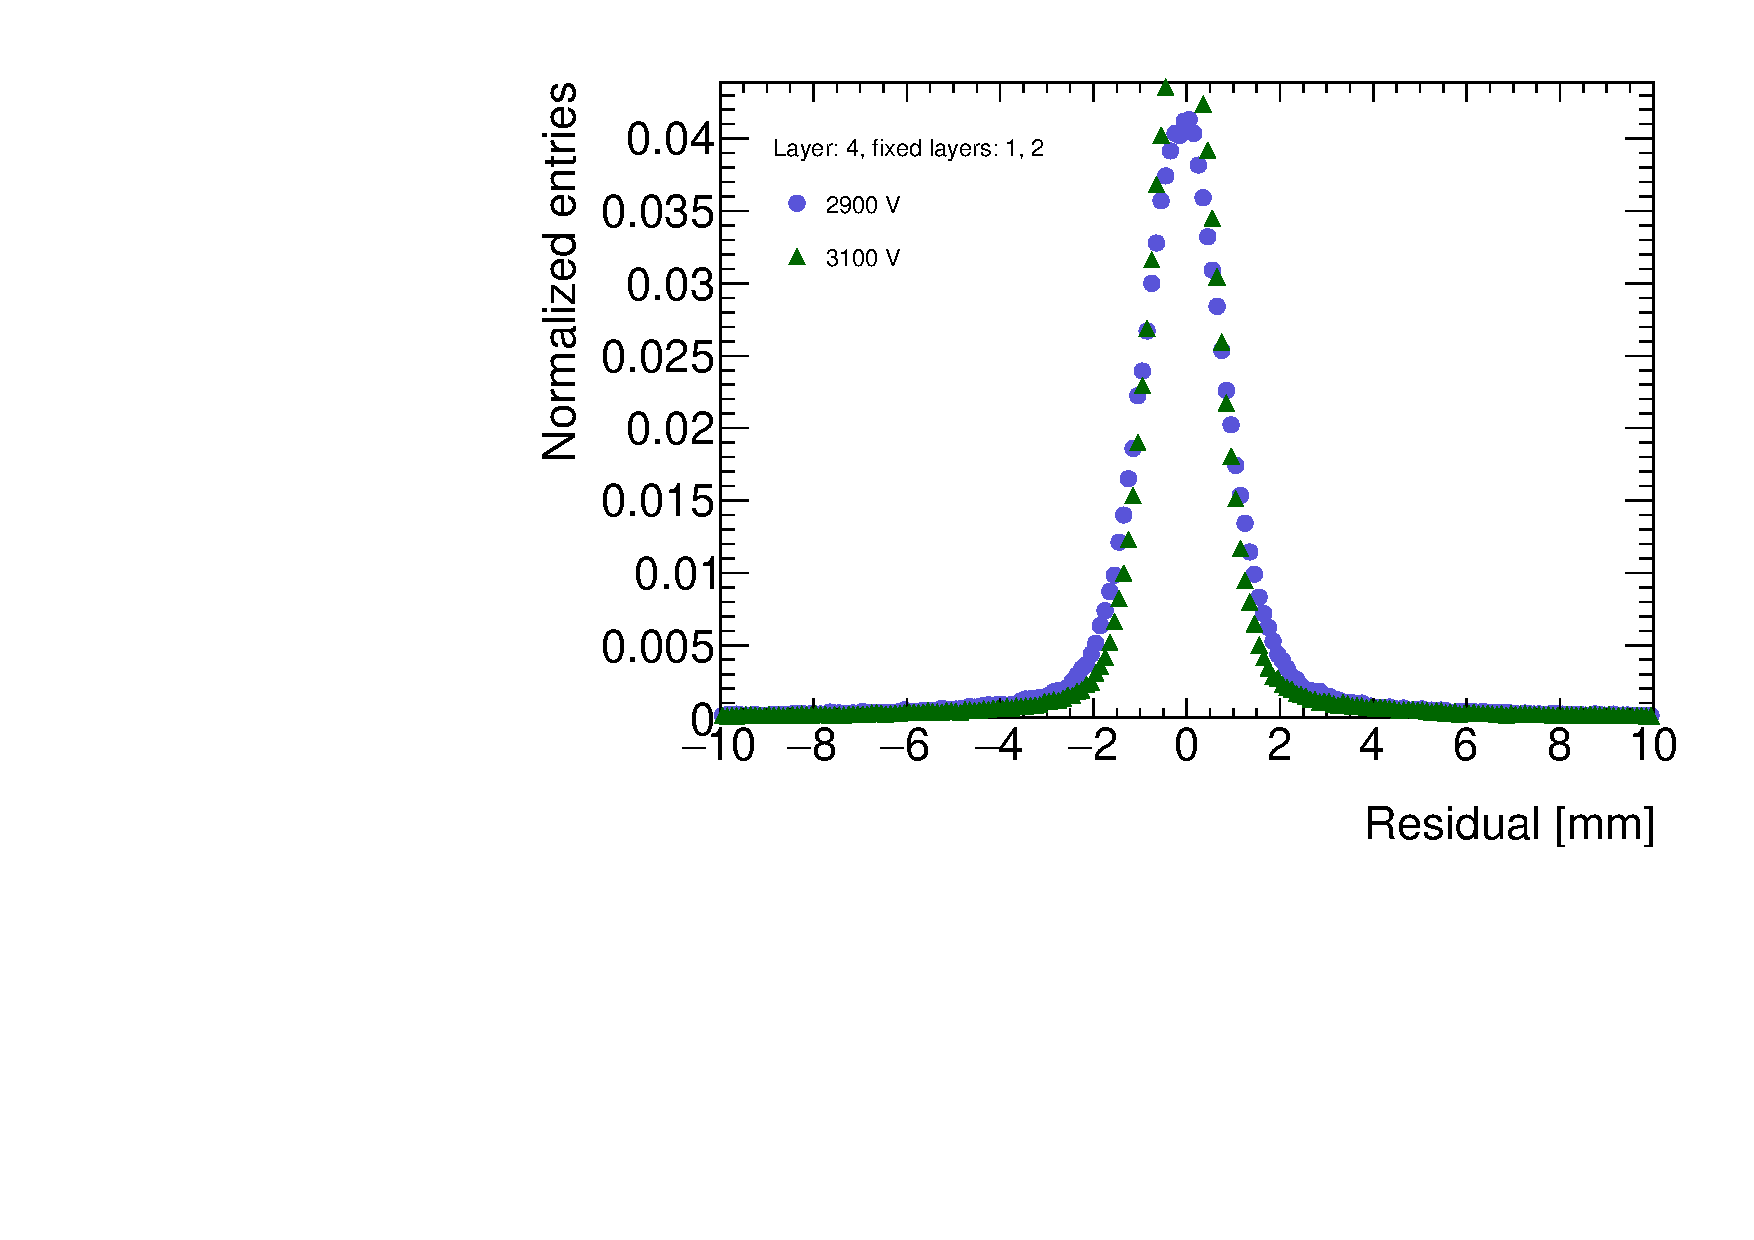
\includegraphics[width = 0.7\textwidth]{figures/figure_residual_distributions_blue_QL2P08_2900V_2021-05-21_green_QL2P08_3100V_2021-05-21_layer4_fixedlayers12.pdf}
    \caption{Residual distribution for tracks on layer 4 built from clusters on layers 1 and 2 for sample quadruplet QL2.P.8 for data collected at 2.9~kV and 3.1~kV.}
    \label{fig:res_dist_2900V_3100V_412}
\end{figure}

Neither dataset is better for calculating the mean of residuals in a given area, so a systematic uncertainty can be assigned based on the difference in residual means calculated for 2.9~kV and 3.1~kV data per tracking combination. For each tracking combination, the difference in the fitted track residual means in \SI{100}{mm} by \SI{100}{mm} areas for 2.9~kV and 3.1~kV data are put in a distribution for a sample quadruplet, as shown in Figure~\ref{fig:voltage_compare_fits}. The means of the distributions for both tracking combinations are near zero, so as expected the collection voltage introduces no bias. Tracks built from clusters on layers 1 and 2 and extrapolated to layer 4 have the worst lever arm and hence the largest root-mean-square (RMS) of \SI{100}{\micro\meter}. The width of the distributions for geometrically favourable tracking combinations are much narrower. The narrowest width of the residual mean difference distribution is for tracks on layer 2 built from clusters on layers 1 and 3 (see Figure~\ref{fig:voltage_compare_fits_213}), with a value of \SI{20}{\micro\meter}.

\begin{figure}
\centering
\begin{subfigure}{.45\textwidth}
  \centering
  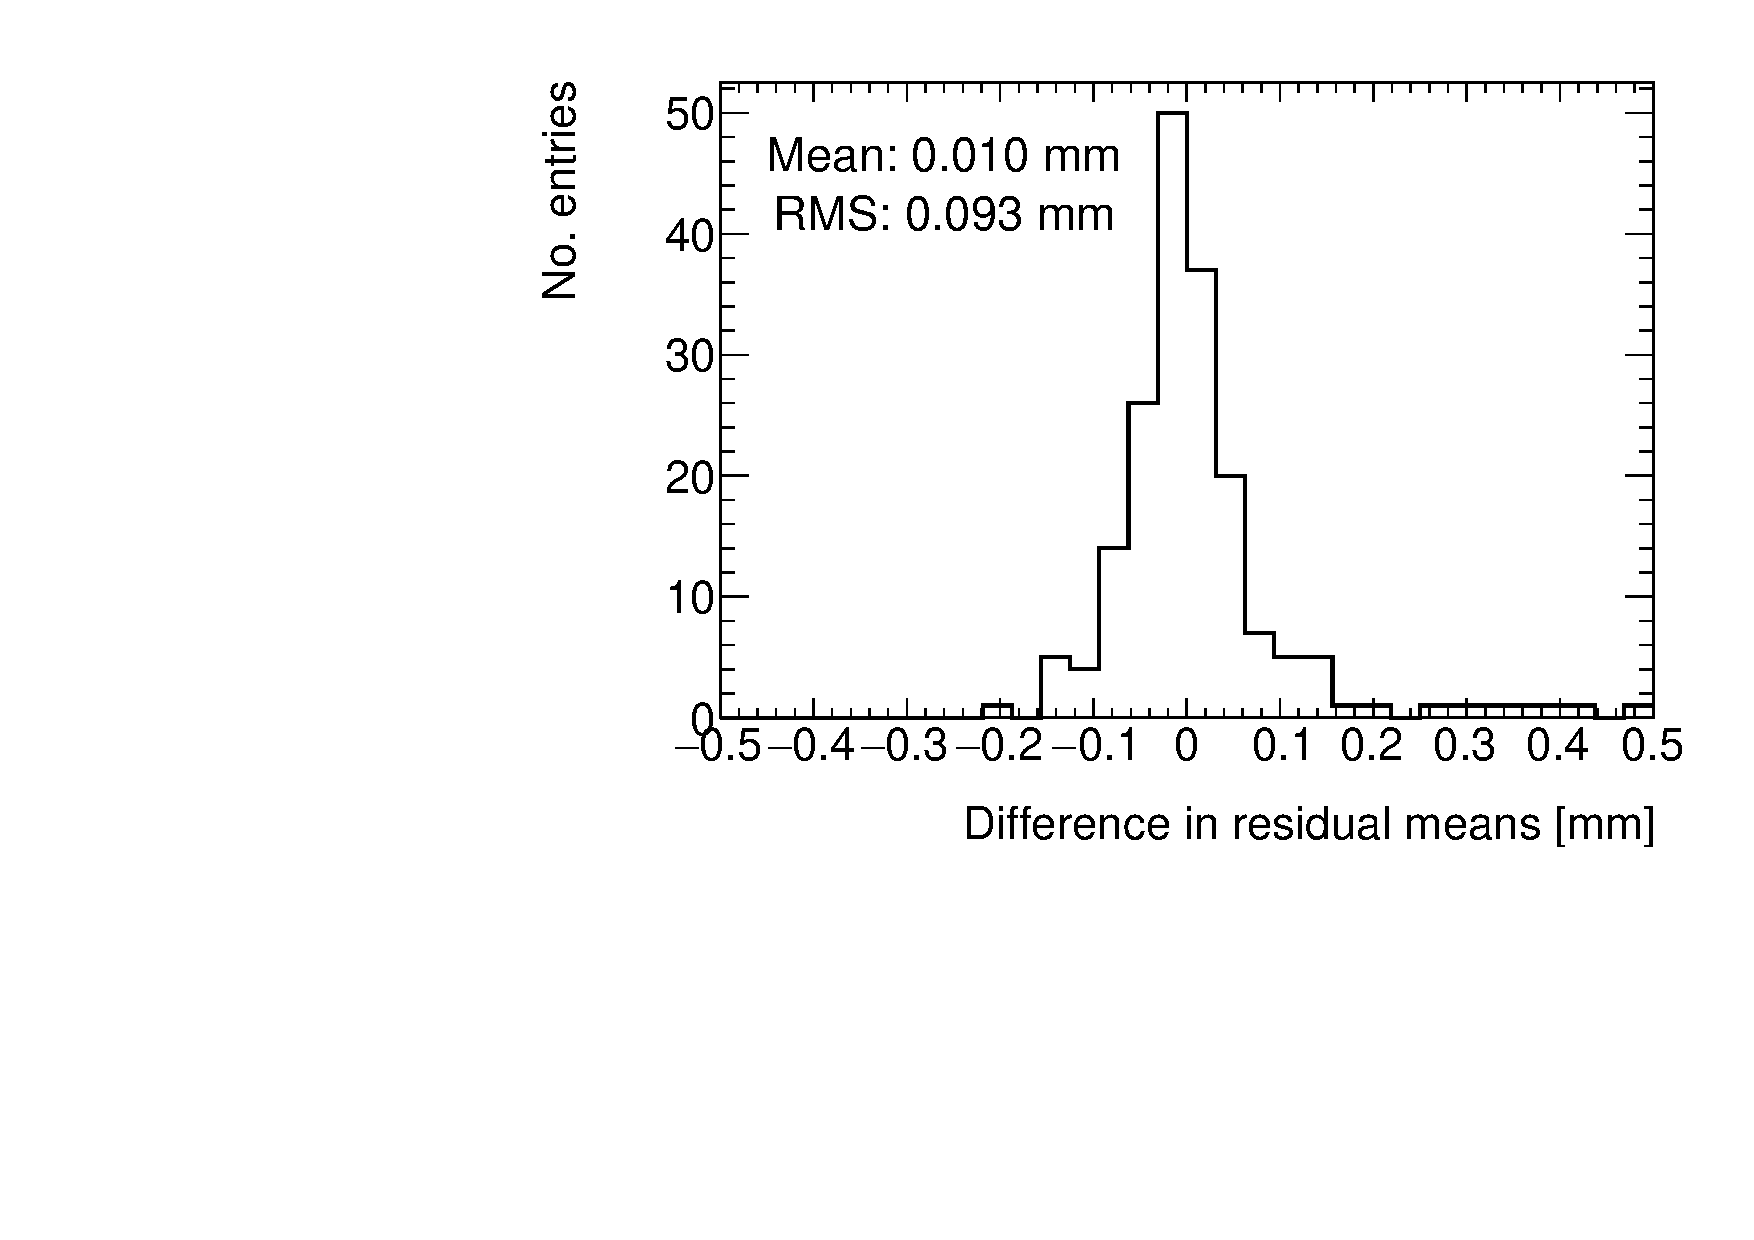
\includegraphics[width=0.97\linewidth]{figures/figure_compare_residual_fits_QL2P08_2900V_2021-05-21_minus_QL2P08_3100V_2021-05-21_layer4_fixedlayers12_mean_differences.pdf}
  \caption{Difference in residual means when measured with residuals on layer 4 built from clusters on layers 1 and 2.}
  \label{fig:voltage_compare_fits_412}
\end{subfigure}\hfill
\begin{subfigure}{.45\textwidth}
  \centering
  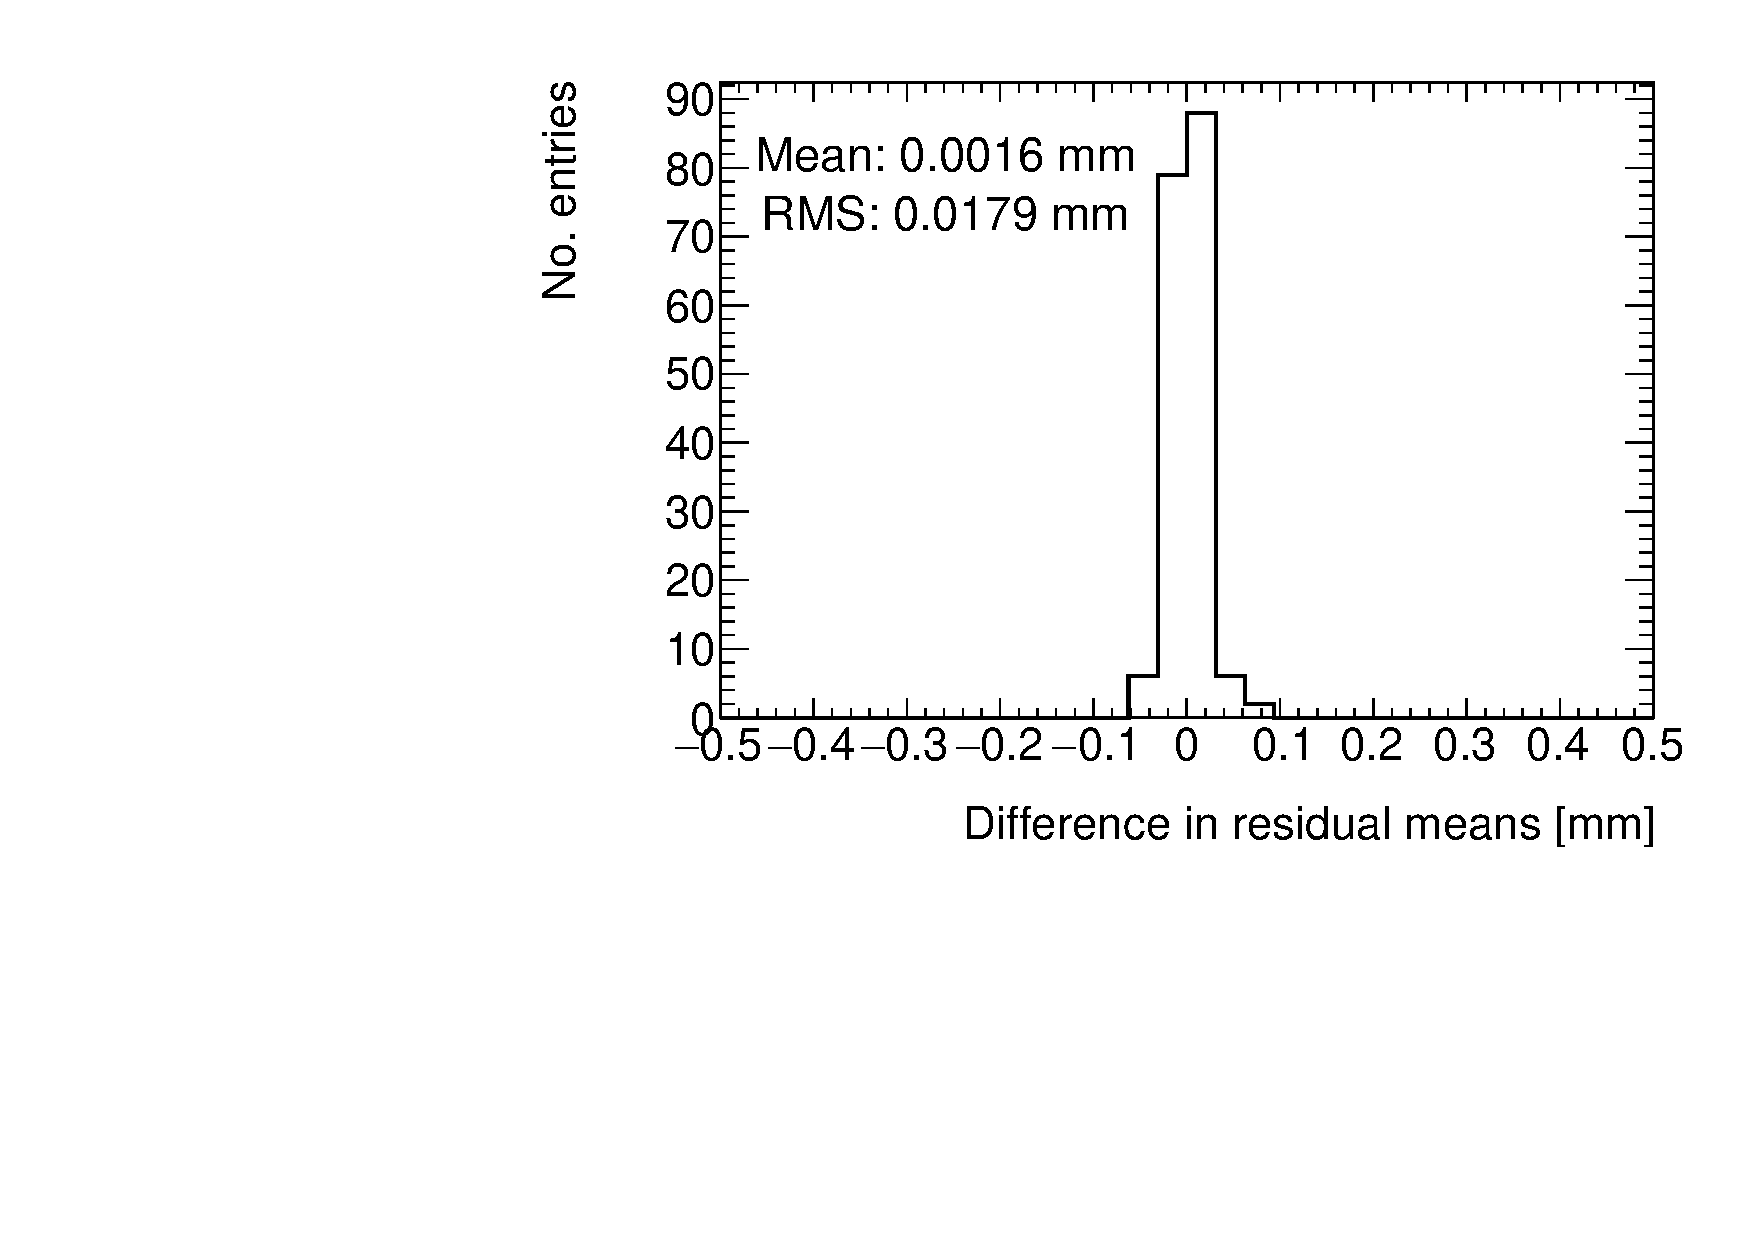
\includegraphics[width=0.97\linewidth]{figures/figure_compare_residual_fits_QL2P08_2900V_2021-05-21_minus_QL2P08_3100V_2021-05-21_layer2_fixedlayers13_mean_differences.pdf}
  \caption{Difference in residual means when measured with residuals on layer 2 built from clusters on layers 1 and 3.}
  \label{fig:voltage_compare_fits_213}
\end{subfigure}\hfill
\caption{Difference in residual means for data collected with sample quadruplet QL2.P.8 at 2.9~kV and 3.1~kV respectively in \SI{100}{\milli\meter} by \SI{100}{\milli\meter} bins.}
\label{fig:voltage_compare_fits}
\end{figure}

% Effect of reclustering on residual means
% --------------------------------------------------
\section{Cluster fit algorithm}
% --------------------------------------------------
\label{appendix:systematics_cluster_fit_fcn}
To ensure that changing the cluster fitting algorithm like in Appendix~\ref{appendix:clustering} would not change the calculated mean of residuals in each region of interest significantly, the residual means were compared in both cases. The distribution of the difference in residual means is plotted in Figure~\ref{fig:cluster_fit_res_mean_compare_fits} for the tracking combinations with the worst and most favourable extrapolation lever arms.

\begin{figure}
  \centering
    \begin{subfigure}{.45\textwidth}
      \centering
      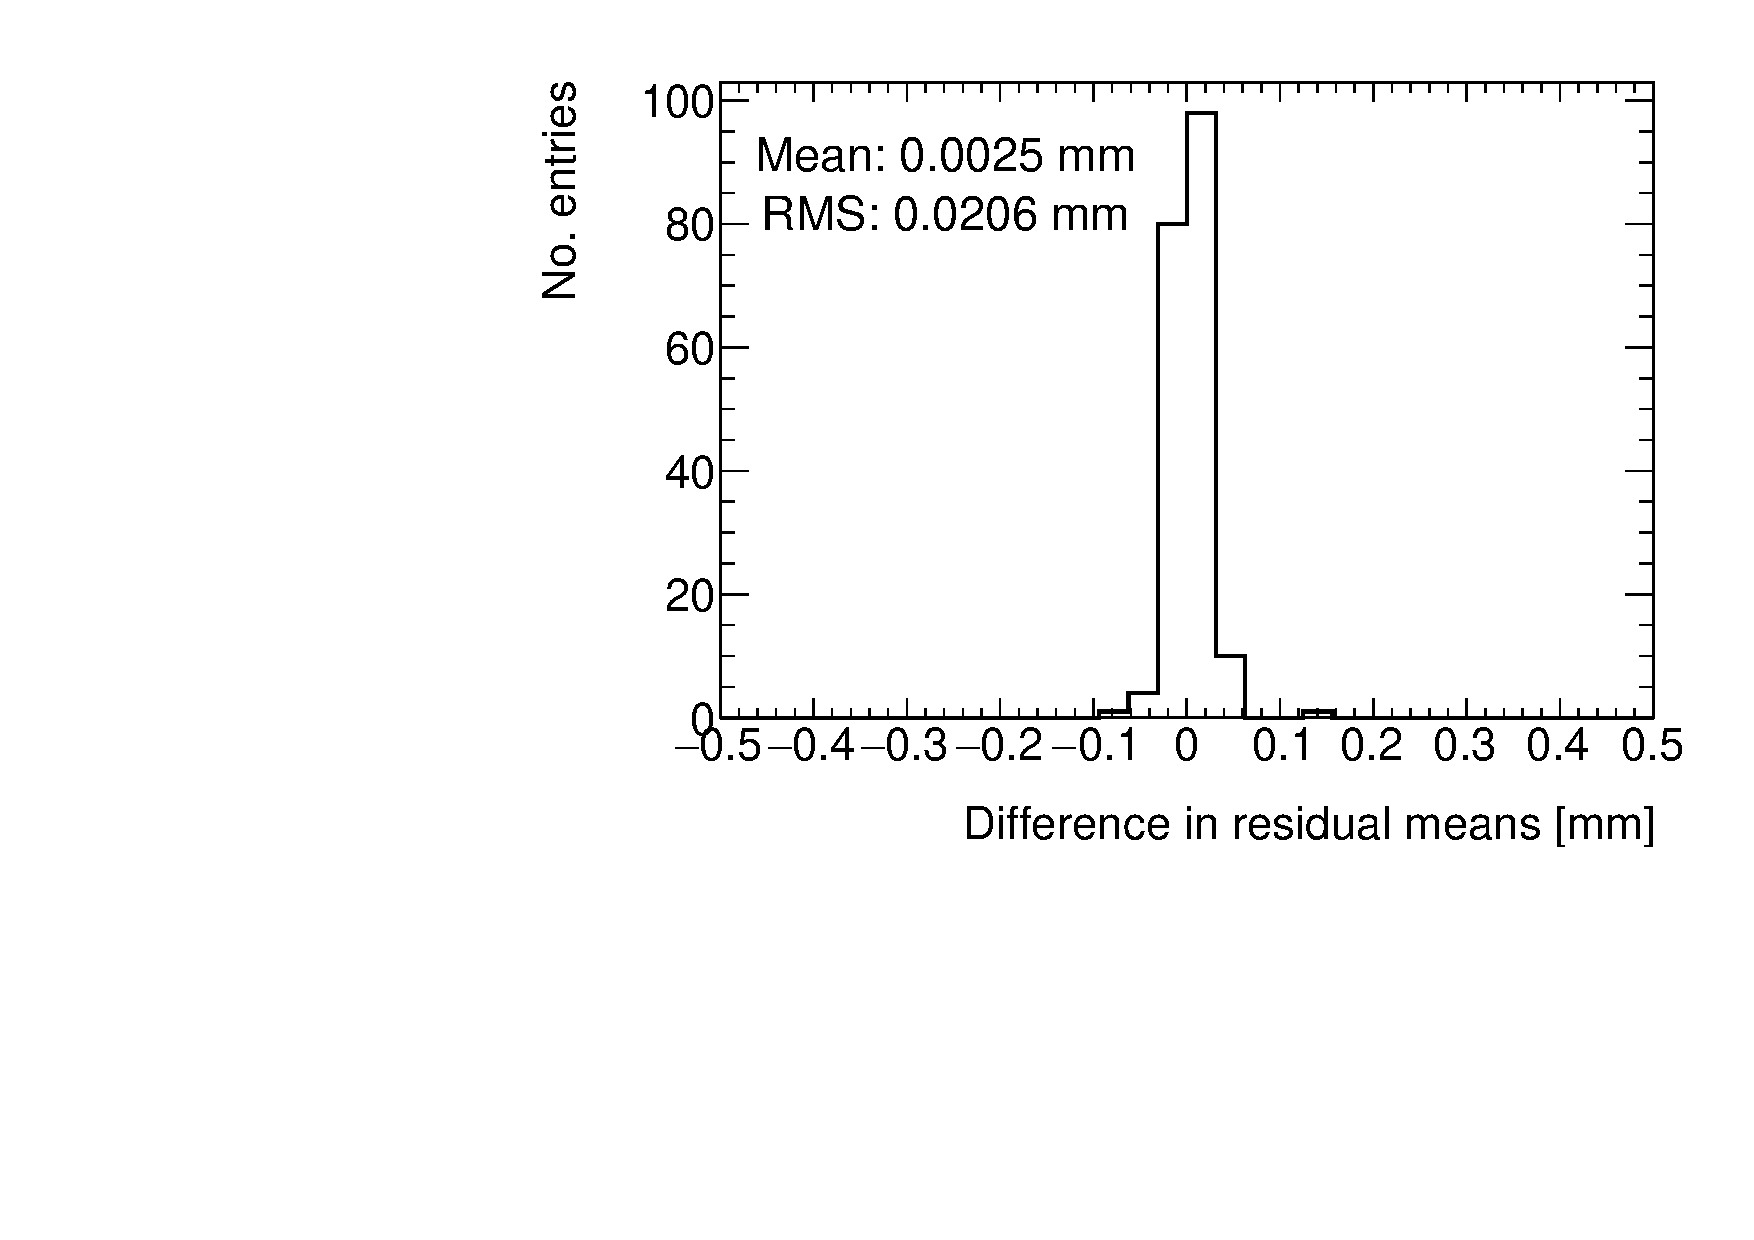
\includegraphics[width=\linewidth]{figures/compare_residual_fits_QL2P08_3100V_2021-06-18_no_dnl_minus_QL2P08_3100V_2021-07-21_no_reclustering_layer4_fixedlayers12.pdf}
      \caption{Difference in residual means when measured with residuals on layer 4 built from clusters on layers 1 and 2.}
      \label{fig:cluster_fit_res_mean_compare_fits_412}
    \end{subfigure}\hfill
    \begin{subfigure}{.45\textwidth}
      \centering
      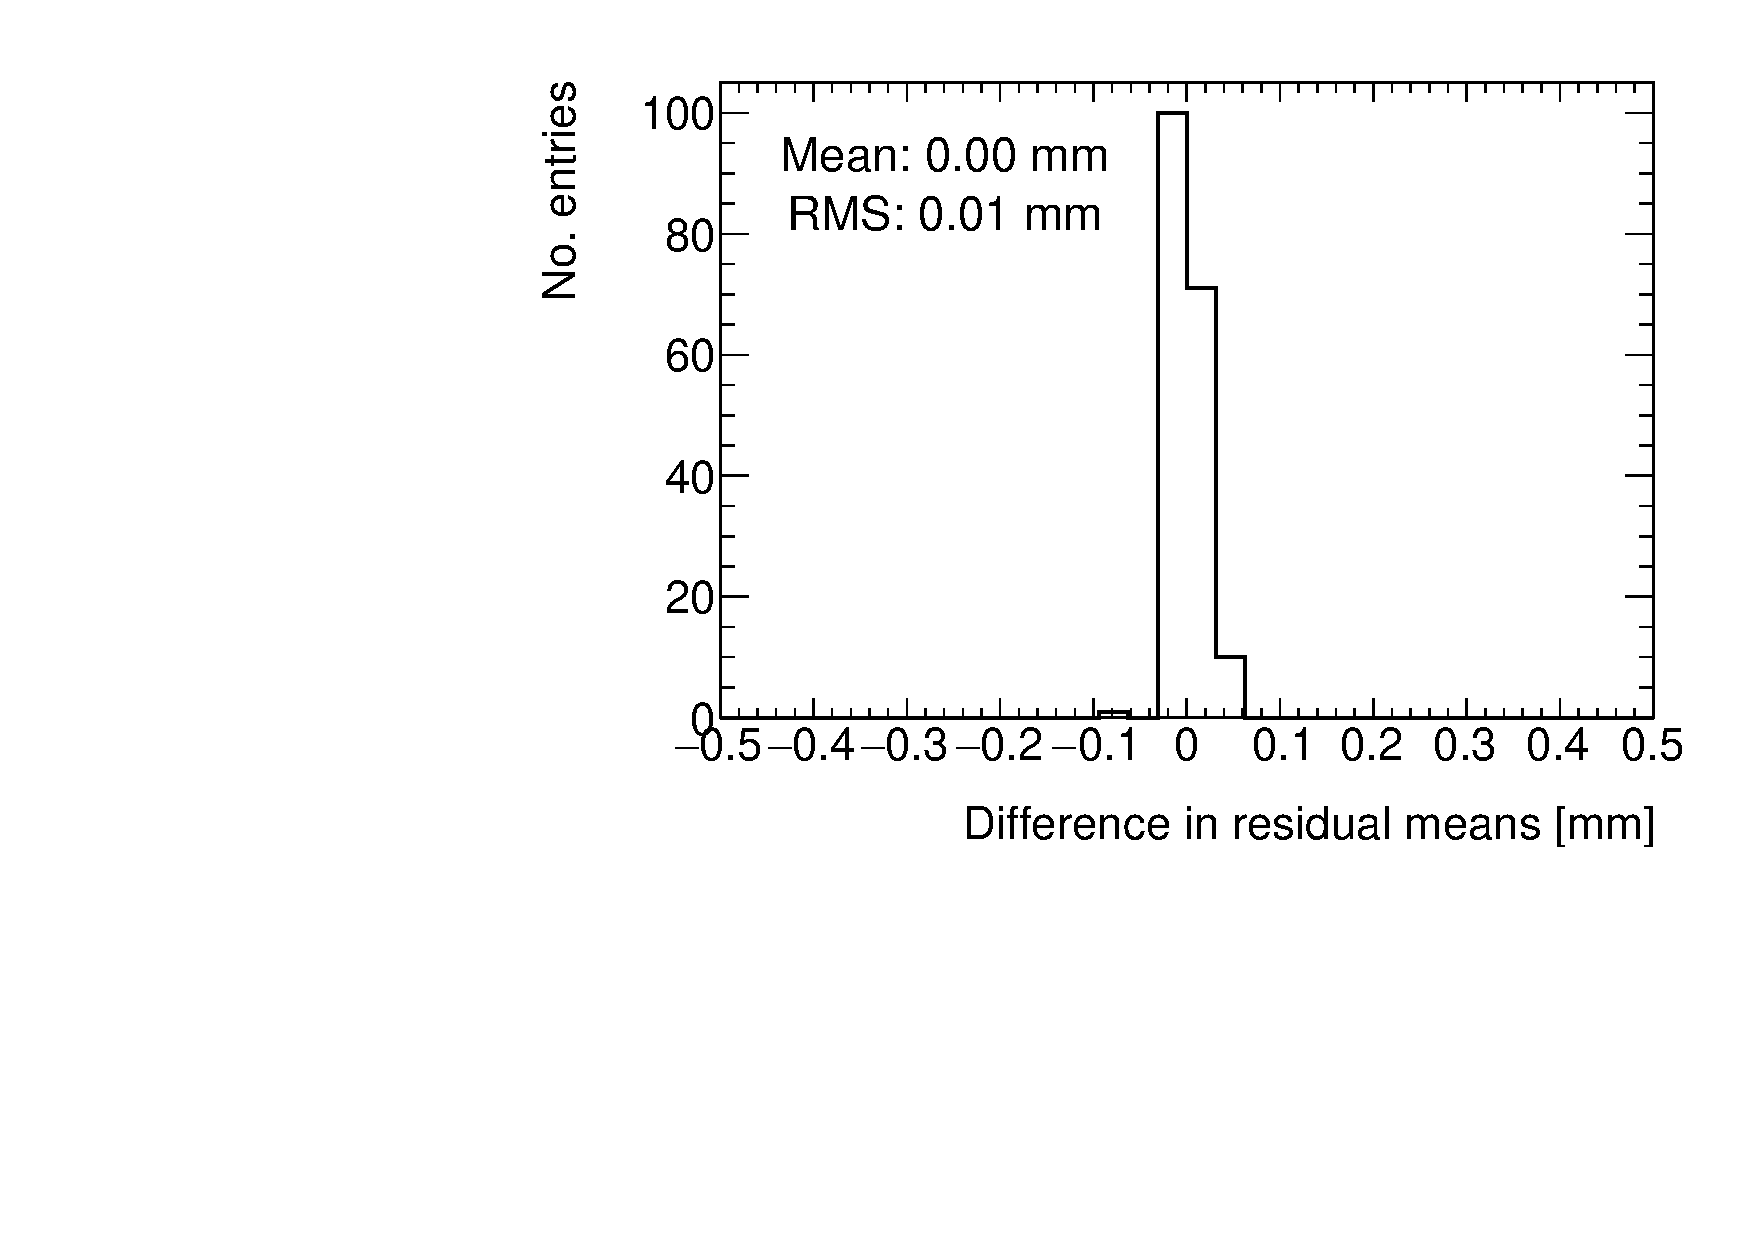
\includegraphics[width=\linewidth]{figures/figure_compare_residual_fits_QL2P08_3100V_2021-06-18_no_dnl_minus_QL2P08_3100V_2021-07-21_no_reclustering_layer2_fixedlayers13.pdf}
      \caption{Difference in residual means when measured with residuals on layer 2 built from clusters on layers 1 and 3.}
      \label{fig:cluster_fit_res_mean_compare_fits_213}
    \end{subfigure}\hfill
  \caption{Difference in residual means when the cluster fit algorithm is \package{Minuit2}~\cite{hatlo_developments_2005} versus Guo's method~\cite{guo_simple_2011} for two different tracking combinations for sample quadruplet, QL2.P.8.}
  \label{fig:cluster_fit_res_mean_compare_fits}
\end{figure}

The mean of the distributions are centered around zero, so the choice of cluster fit algorithm did not introduce any bias. Differences on the order of \SI{50}{\micro\meter} are important, so the root-mean-squares (RMS's) of the distributions show that the clustering algorithm had a small but notable effect between 10-\SI{20}{\micro\meter} from the most to least geometrically favourable tracking combinations. Therefore, the RMS for each tracking combination will be used to add a systematic uncertainty on the residual means accounting for the effect that different cluster fit algorithms have on the residual means.

% --------------------------------------------------
\section{Differential non-linearity}
% --------------------------------------------------
\label{appendix:systematics_dnl}
% Edit count: 1

\paragraph*{Definition} \hfill \break
In this context, differential non-linearity (DNL) is when the reconstructed cluster mean is biased by the fit of the discretely sampled peak signal amplitude distribution over the strips. The bias depends on the relative position of the avalanche with respect to the center of the closest strip. For a summary of DNL, refer to page 40 of~\cite{lefebvre_thesis}, an early paper studying its effects~\cite{endo_systematic_1981}, and for an example application, refer to~\cite{abusleme_performance_2016}. 

\paragraph*{Application and effect of DNL} \hfill \break
The cluster mean was corrected for DNL using the equation:

\begin{equation}
\label{eqn:dnl_corr}
y' = y + a \sin \left( 2 \pi y_{rel} \right)
\end{equation}

where $y$ is the cluster mean, $y_{rel}$ is the relative position of the cluster mean with respect to the strip's center, $a$ is the amplitude of the correction, and $y'$ is the corrected cluster mean. The amplitude can be derived by comparing the reconstructed hit position to the expected hit position, as done in~\cite{abusleme_performance_2016}. With cosmic muons, there is no reference hit position to compare to, so track residuals were used as a proxy \cite{lefebvre_thesis}. The hallmark of the DNL effect is the periodic pattern in the residual versus $y_{rel}$ profile, and the effect of correcting the cluster means using an amplitude of \SI{50}{\micro\meter} is shown in Figure~\ref{fig:dnl_corr_effect}. An amplitude of \SI{50}{\micro\meter} is based on Dr. Lefebvre's~\cite{lefebvre_thesis} estimate of the DNL amplitudes by layer, quadruplet and cluster size using cosmic muon tracks~\cite{lefebvre_thesis}. Little variation is seen in the amplitude parameters with respect to the quadruplet tested, the layer and the cluster size so a universal correction is used.
%TODO How little is little? Check your notes.
%TODO exclusive better be defined somewhere clearly.

\begin{figure}
    \centering
    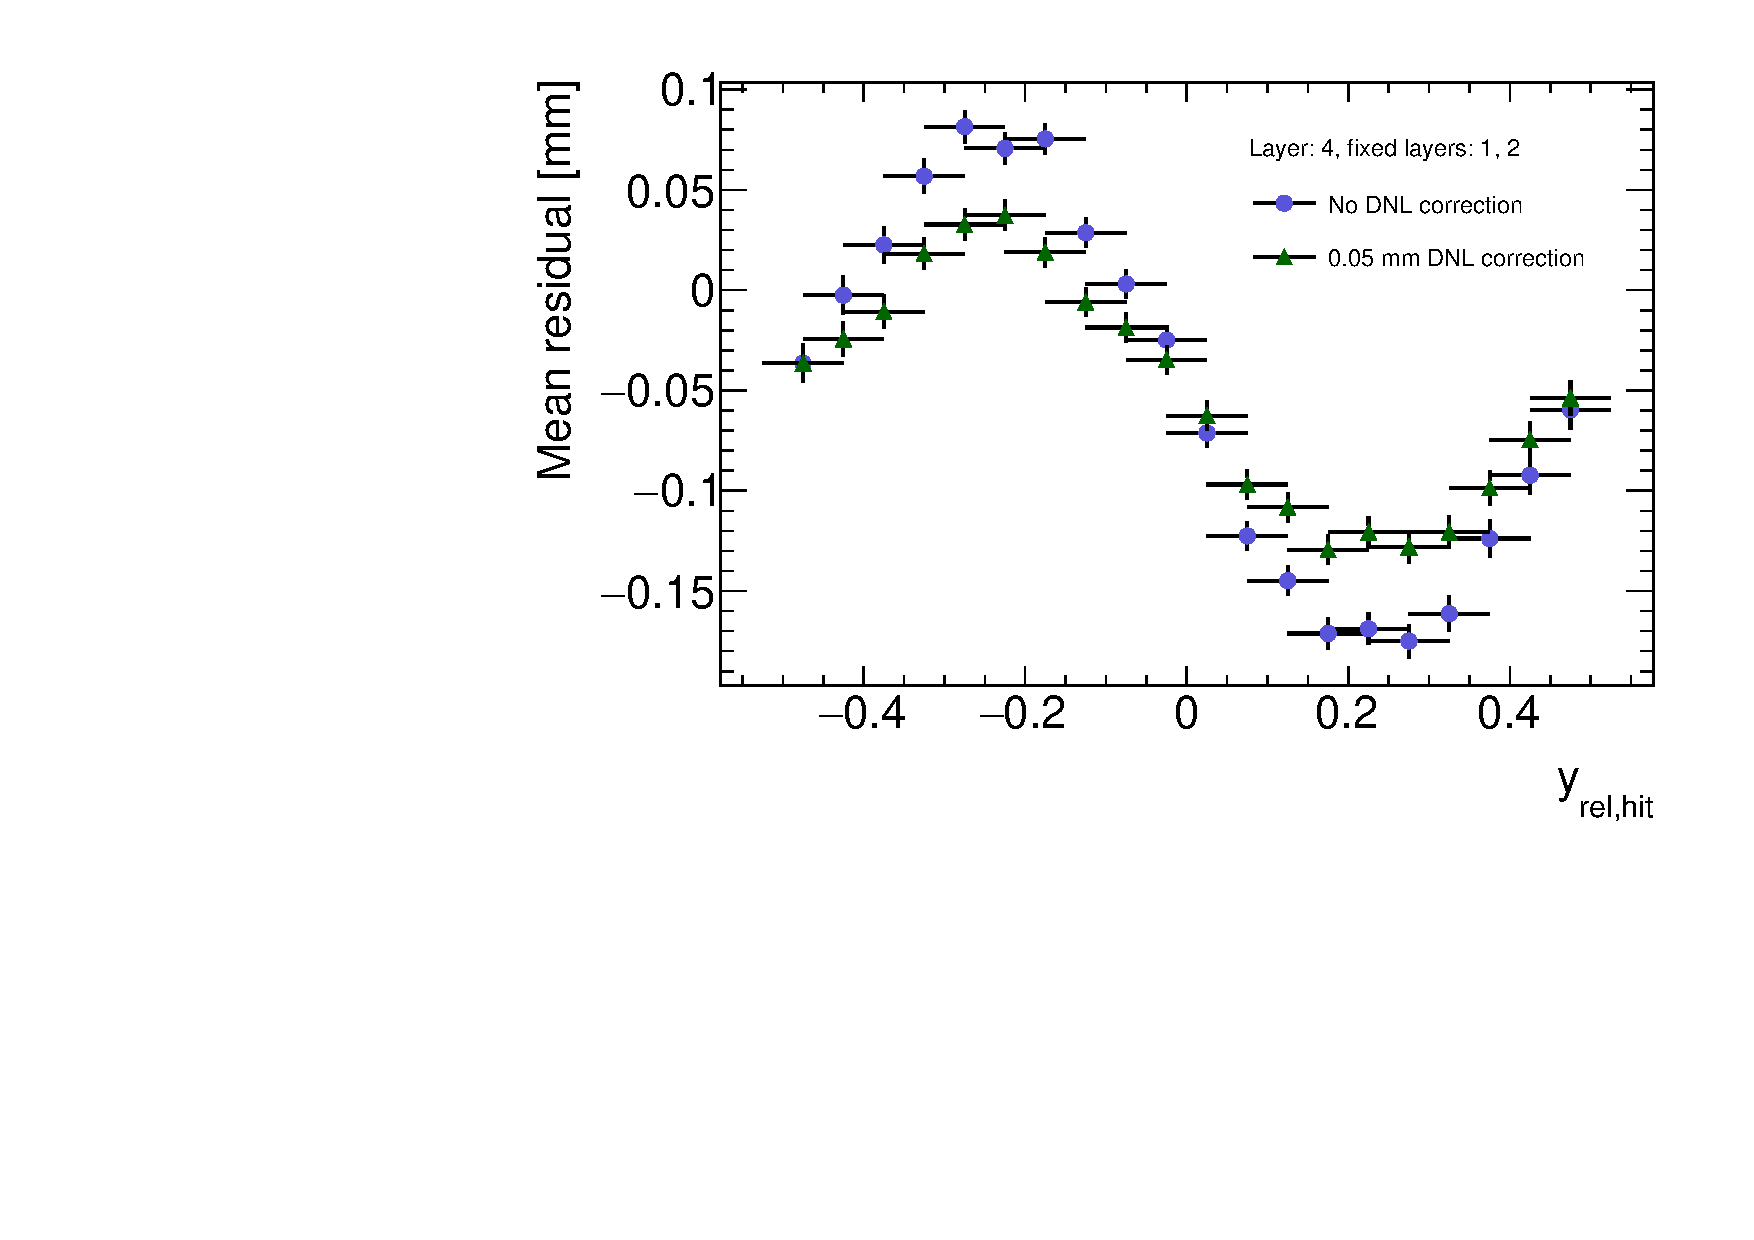
\includegraphics[width = 0.6\textwidth]{figures/figure_dnl_profiles_blue_QL2P08_3100V_2021-06-18_no_dnl_green_QL2P08_3100V_2021-06-18_2_50um_universal_DNL_layer4_fixed12.pdf}
    \caption{Effect applying a \SI{50}{\micro\meter} DNL correction to the profile of the residuals sorted by $y_{rel}$ for residuals built from clusters on layers 1 and 2 and extrapolated to layer 4 of quardruplet, QL2.P.8.}
    \label{fig:dnl_corr_effect}
\end{figure} 

Although the correction is not large enough in this case, the figure shows that the correction does reduce the DNL effect. Slightly better performance is seen in the interpolation tracking combinations where the quality of the residuals is better. DNL corrections for cosmic muon data are difficult because the DNL effect is obscured by the effect of misalignments between strip layers and noise. Misalignments cause the center of the sinusoidal pattern in Figure~\ref{fig:dnl_corr_effect} to be shifted off of zero, since the mean of residuals is shifted.

Figure~\ref{fig:dnl_compare_fits} shows the distribution of the difference in residual means calculated in \SI{100}{mm} by \SI{100}{mm} areas for mean track residuals on layer 4 obtained using layers 1 and 2 as reference. The mean of the distribution is zero within the root-mean-square so the DNL correction does not bias the residual means. It is apparent that the effect of the DNL correction on the residual means is on the order of micrometers given the RMS of \SI{10}{\micro\meter} in the worst extrapolation case. Although the $\sigma$'s of the residual distributions shrink with the DNL correction, the mean is the parameter of interest so the bias in the fitted $\sigma$'s was ignored. Therefore, in this analysis DNL is not corrected for. 

\begin{figure}
    \centering
    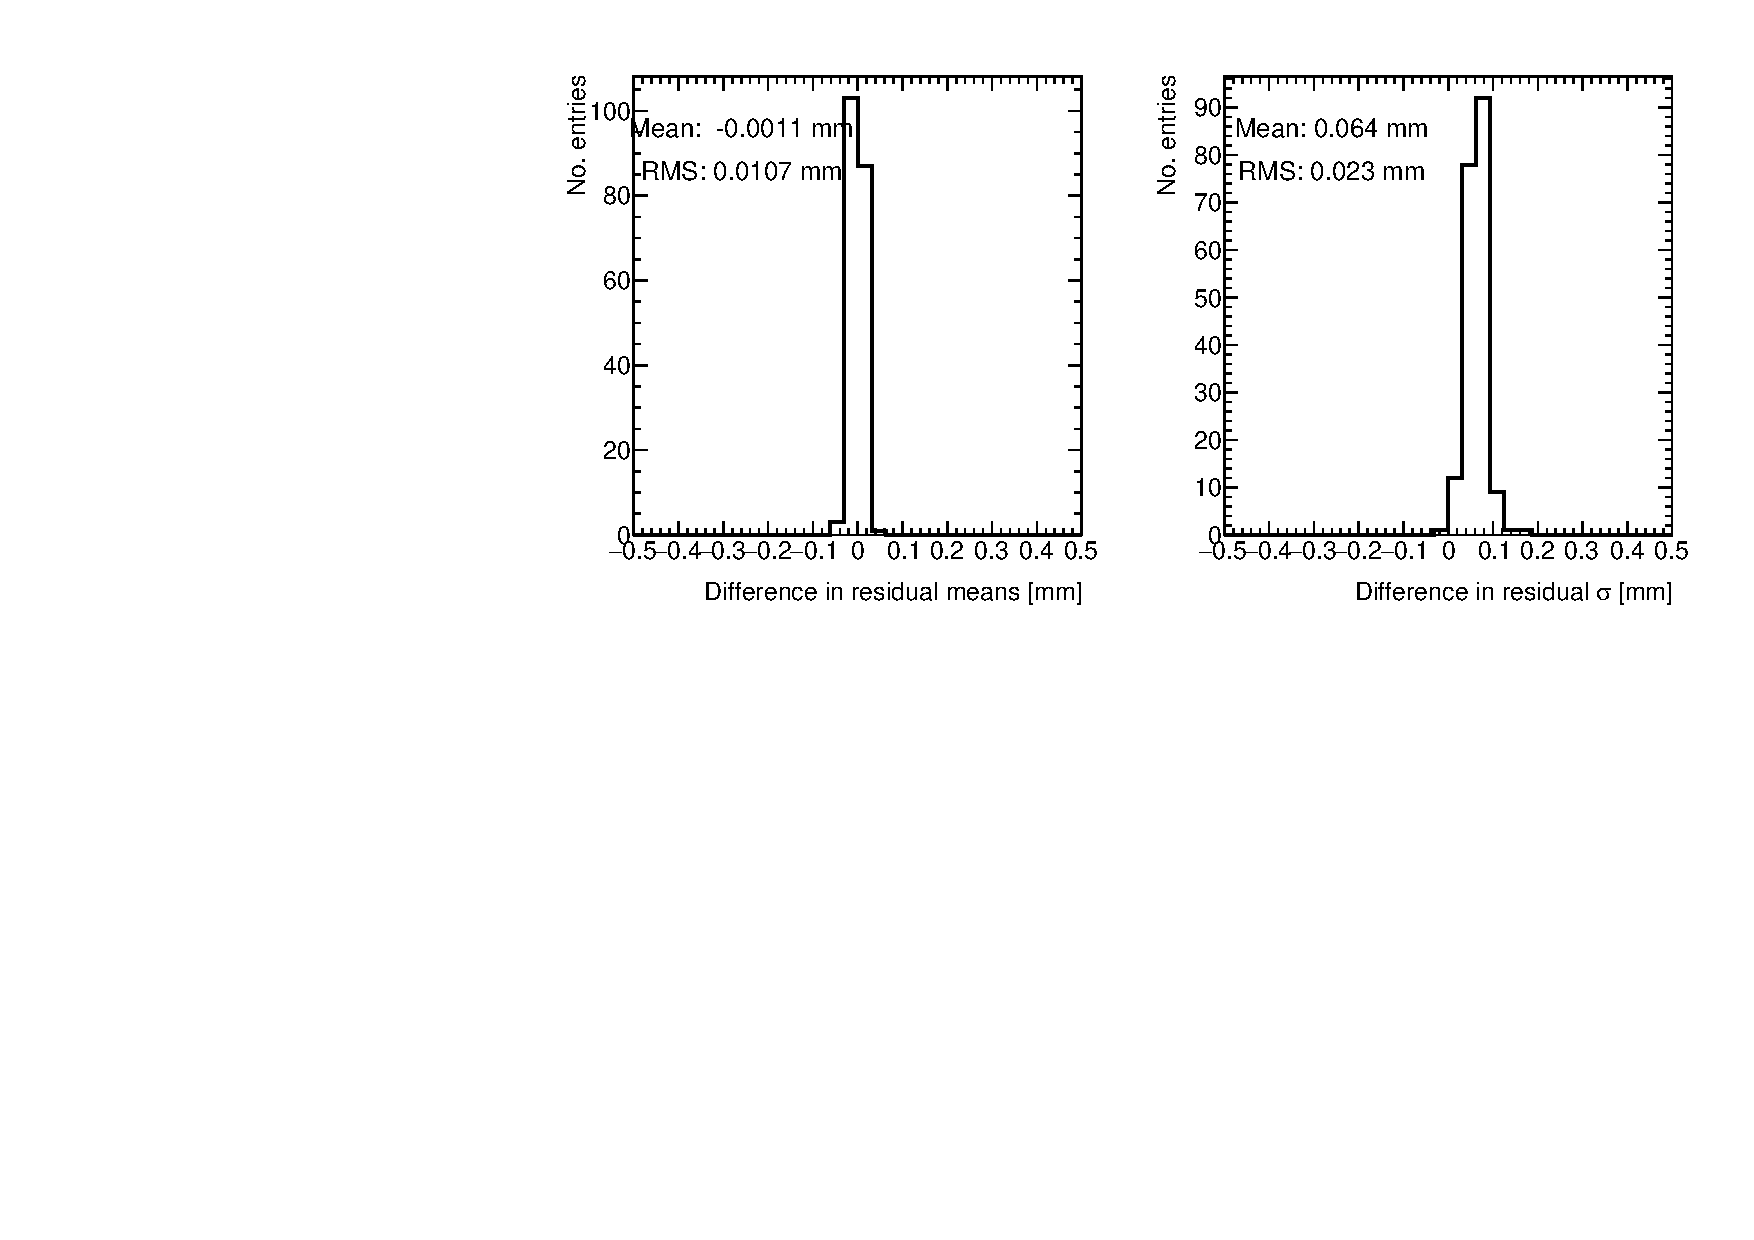
\includegraphics[width = \textwidth]{figures/figure_compare_residual_fits_QL2P08_3100V_2021-06-18_no_dnl_minus_QL2P08_3100V_2021-06-18_2_50um_universal_DNL_layer4_fixedlayers12.pdf}
    \caption{Difference in residual distribution means and $\sigma$'s with and without DNL correction for residuals on layer 4 obtained using reference layers 1 and 2 for sample quadruplet, QL2.P.8.}
    \label{fig:dnl_compare_fits}
\end{figure}
